\documentclass[12pt,letterpaper,titlepage]{article}

\usepackage{fontspec}
\defaultfontfeatures{Mapping=tex-text}
\usepackage{xunicode}
\usepackage{xltxtra}
\usepackage{amsmath}
\usepackage{pdfpages}
\usepackage{amsfonts}
\usepackage{bbold}
\usepackage{amssymb}
\setcounter{secnumdepth}{0}
\usepackage{nameref}
\usepackage{enumitem}
\usepackage{environ}
\usepackage{pgfplots}

\showboxdepth=\maxdimen
\showboxbreadth=\maxdimen


\usepackage{paracol}
\usepackage{wrapfig}
\globalcounter{table}
\globalcounter{figure}
\usepackage{graphicx}
\usepackage[left=1in,right=1in,top=1in,bottom=1in]{geometry}
\graphicspath{{img/}}

\author{Jacob Abel}
\title{	Design \& Simulate 4 Ex1.6
	\\\large ECE2204 CRN:82929
}

\setlength{\parskip}{0.5em}

\begin{document}
\maketitle
\begin{raggedright}

\section{Problem 4.6.a.1: }
\subsection{Design}

Consider a silicon pn junction at $T = 300 K$ with a donor doping concentration of $N_d = 10^{14} cm^{-3}$, and at $V_R = 3V$ the junction capacitance is $C_j = 0.245 pF$. Assume that the Boltzmann constant is $k=86\times 10^{-6} eV/K$, the electron charge is $e = 1.6 \times 10^{-19} C$, $n_i = 2.3 \times 10^{10} cm^{-3}$ and $C_{j0} = 0.7 pF$. Assume $\mathbb{e}$ is the exponential. Find the acceptor doping concentration $N_a$.


\begin{equation}\scalebox{1.25}{
$
V_{bi} = \frac{kT}{e}\ln(\frac{N_aN_d}{n_i^2}) 
\implies N_a = \frac{n_i^2}{N_d}\mathbb{e}^{(\frac{e\times V_{bi}}{kT})}
$
}
\end{equation}
\begin{equation}\scalebox{1.25}{
$
C_j = C_{j0}(1 + \frac{V_R}{V_{bi}})^{-1/2} 
\implies V_{bi} = \frac{V_R}{(\frac{C_j}{C_{j0}})^{-2} - 1}
$
}
\end{equation}
\begin{equation}\scalebox{1.25}{
$
V_{bi} = \frac{3V}{(\frac{0.245pF}{0.7pF})^{-2} - 1} = 0.42V
$
}
\end{equation}
\begin{equation}\scalebox{1.25}{
$
N_a = \frac{(2.3 \times 10^{10} cm^{-3})^2}{10^{14} cm^{-3}}\mathbb{e}^{(\frac{1.6 \times 10^{-19} C\times0.42V}{300K \times 86\times 10^{-6} eV/K})} = 6.078\times 10^{13} cm^{-3}
$
}
\end{equation}

The acceptor doping concentration is $N_a = 6.078\times 10^{13} cm^{-3}$.
	
\subsection{Validation}

I was not able to get LTSpice to generate a validation simulation with $N_a$ as my dependent value. As a result there is no validation simulation. 

\textbf{Note to grader:} If you know how to get LTSpice to simulate with $N_a$ as the dependent variable and $V_R$ as the driving independent variable, I would be very appreciative if you could leave me a comment as as to how. Despite being generally decent with LTSpice I could not make it work this time around.

\clearpage
\section{Problem 4.6.b.1: } Derived from 1.23 by changing values.
\subsection{Design}
The zero-biased junction capacitance of a silicon pn junction is $C_{j0} = 0.5 pF$. The doping concentrations are $N_a = 1.2 \times 10^{16} cm^{-3}$ and
$N_d = 5 \times 10^{15} cm^{-3}$. Assume $n_i = 1.5 \times 10^{10} cm^{-3}$. Determine the junction capacitance at $V_R = 2V$.

\begin{equation}\scalebox{1.25}{
$
V_{bi} = \frac{300K \times 86\times 10^{-6} eV/K}{1.6 \times 10^{-19} C}\ln(\frac{1.2 \times 10^{16} cm^{-3} \times 5 \times 10^{15} cm^{-3}}{(1.5 \times 10^{10} cm^{-3})^2}) = 0.6797V
$
}
\end{equation}
\begin{equation}\scalebox{1.25}{
$
C_j = 0.5pF (1 + \frac{2V}{0.6797V})^{-1/2} = 0.252pF
$
}
\end{equation}

The junction capacitance at $V_R = 2V$ is $C_j = 0.252pF$

\subsection{Validation}

\begin{center}
LTSpice Implementation (accurate with $< 1\%$ deviation from design result)
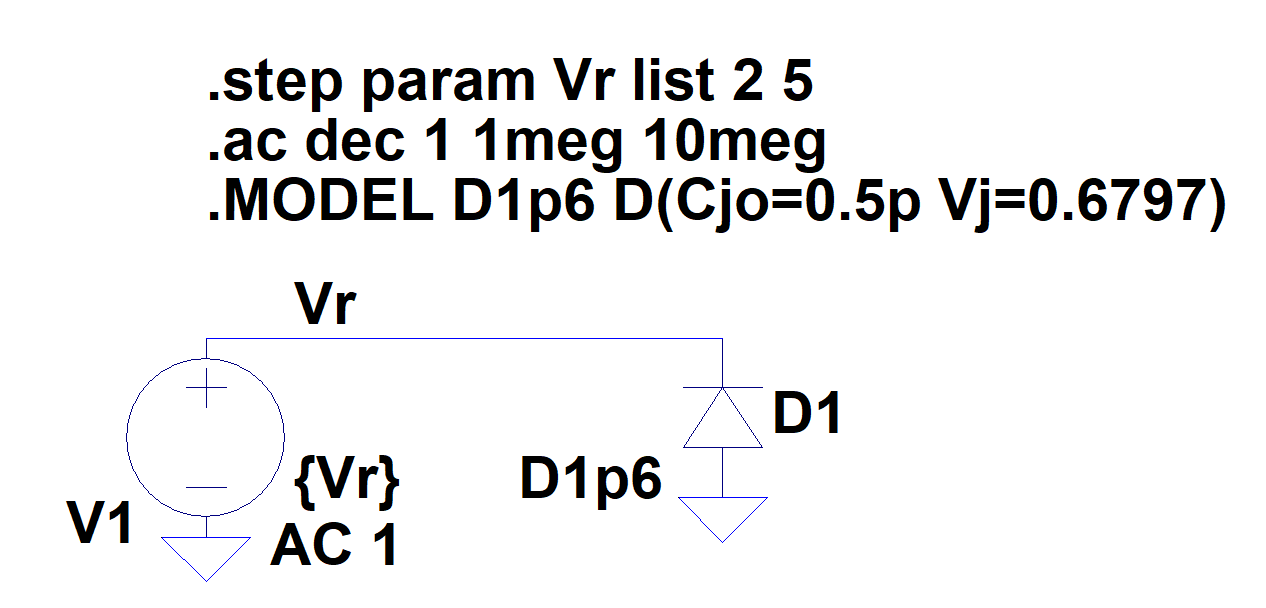
\includegraphics[width=.49\textwidth, height=\textheight, keepaspectratio=true]{ds2b}
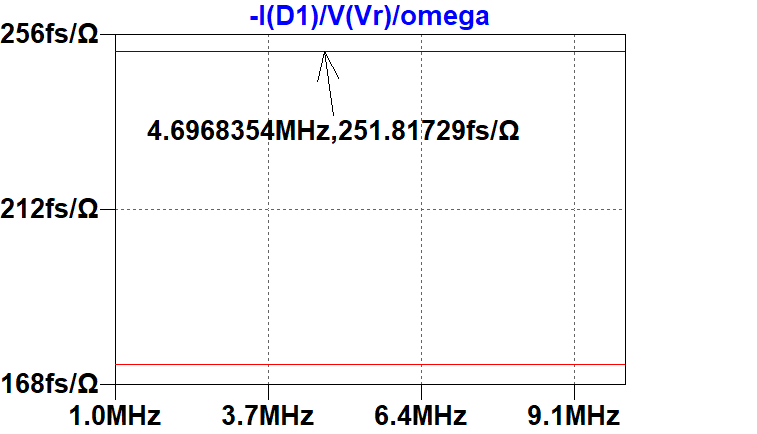
\includegraphics[width=.49\textwidth, height=\textheight, keepaspectratio=true]{ds2c}
$Err = \frac{|252-251.8|}{252} = 0.00079 = 0.079\%$
\end{center}

This assignment demonstrates an understanding of basic pn junction theory, the equations, and derivations necessary to solve for parameters essential to the function of pn junctions.

\textit{I have neither given nor received unauthorized assistance on this assignment.}


\end{raggedright}
\end{document}
